\chapter{Neuroimaging applications}
\label{ch:neuroimaging}
The neuroimaging community developed multiple ways of capturing, processing, and 
analyzing brain data to study the brain and diagnose patients in clinics.
This chapter discusses the three magnetic resonance imaging (MRI) modalities for 
neuroimaging and associated pipelines to process them and more recent machine learning techniques for neuroimaging.
Finally, it discusses the potential of using reduced precision techniques for neuroimaging tools.

\section{MRI processing}
\label{sc:preprocessing}
Magnetic resonance imaging (MRI) is a standard tool used by neuroscientists to
perform clinical diagnoses and for researchers to better understand the brain. 
With the evolution of MRIs, three modalities emerged: structural MRI,
functional MRI (fMRI), and diffusion MRI (dMRI).\
While other modalities such as EEG, CT, and PET exist, we focus on MRI data types
for their non-intrusive property.
MRI analyses are technically challenging to process due to the complexity of the
pre-processing steps and the extensive data size produced as output and during intermediary steps.
In this section, we briefly introduce these different MRI modalities.
Moreover, we will explore pre-processing steps to analyze the data and
describe standard software toolkits to perform the pre-processing and analysis for
each modality.

Structural, or anatomical, MRI is a classical method that is vastly used in clinical diagnosis.
Structural MRI aims to provide static information on the anatomy of the brain.
The use of T1-weighted and T2-weighted images allows for the diagnosis and
monitoring in applications such as epilepsy, Parkinson's disease, acute cerebral
hemorrhage, and multiple sclerosis ~\cite{Symms2004-xj}.
Capturing data across different individuals, sessions, or even scanner types will often result in a significant variation in brain structure. 
Performing meaningful analysis requires realigning the data into a common space, thus reducing variability.
Two popular methods are \textit{volume-based normalization}, which uses a
template to realign an image to the common space, and \textit{surface-based normalization},
which takes advantage of the fully connected topology of the cerebral cortex to
normalize the surface of the brain tissues.

Other standard pre-processing steps for anatomical data are \textit{bias field correction}
to correct the variation in voxel intensity, \textit{brain extraction}, and \textit{tissue segmentation}
to separate the different components such as gray matter, white matter, and cerebrospinal fluid.
FreeSurfer~\cite{Fischl2012-bp} is a toolkit that allows structural MRI pre-processing and analysis.
Its many features include accurate topology correction, surface-based inter-subject
alignment, volume and surface cross-subject registration, and whole-brain segmentation.

Unlike structural MRI, fMRI is used to measure brain activity and connectivity.
fMRI became dominant due to its fundamentally non-invasive acquisition, high spatial
resolution, signal reliability, robustness, and reproducibility~\cite{Soares2016-tz}.
The measurements of fMRI data are based on the concept that neural activation involves
an augmentation in blood flows.
It captures brain images using the blood oxygenation level-dependent (BOLD) contrast methods.
Figure~\ref{fig:fmri_workflow} depicts the key pre-processing steps to correct
for artifacts in the data prior to analysis.
For example, head motion is a critical issue during fMRI acquisition.
A common strategy to correct for it uses a reference volume to realign the data.
Spatial transformation is required to analyze the subject in the same space.
For this step, the volumes are normalized to a template.
Finally, the different sections of brain data are acquired at different time slices.
Performing proper analysis requires the data from the slices to be corrected to interpolate the signal at a particular time point.
Another critical step is spatial smoothing, which averages the data points with their neighbors.
This increases the signal-to-noise ratio for the data and improves statistical tests' results.
Finally, multiple techniques were developed to perform statistical analysis on the pre-processed data of task-based and resting-state studies.
fMRIPrep~\cite{Esteban2019-og} is a toolkit that offers various techniques for the pre-processing steps
and statistical analysis of resting-state and task-based function MRI data.
The data output also creates an HTML report for users to assess the generated data quality.
A combination of a citation boilerplate, thorough documentation, and open-source code
fMRIPrep implementation and processing is transparent and encourages reproducibility. 

\begin{figure}[h]
	\centering
	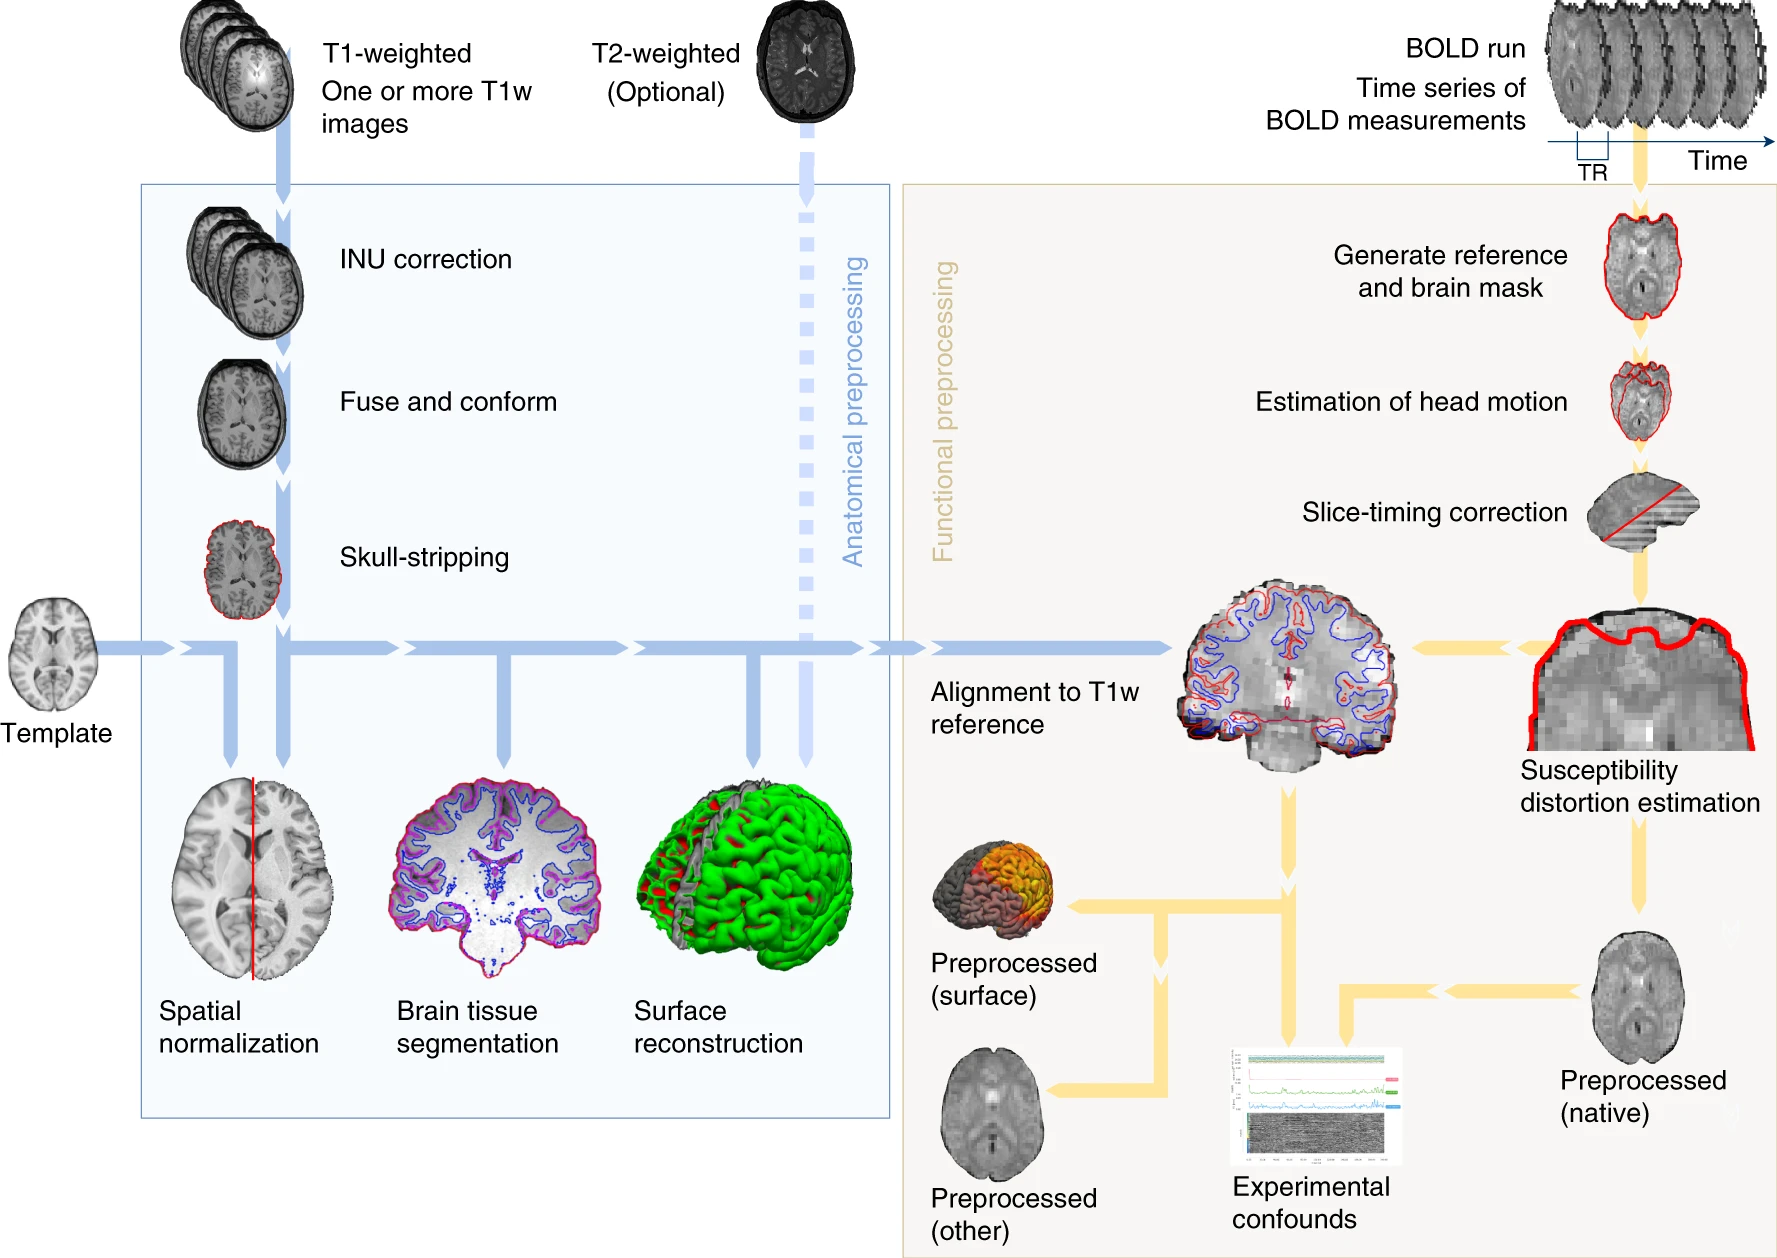
\includegraphics[width=\textwidth]{fMRIPrep_workflow.png}
	\caption{Preprocessing steps for structural and functional MRI data. (Taken from~\cite{Esteban2019-og})}
	\label{fig:fmri_workflow}
\end{figure}

While fMRI uses BOLD signal to capture data, dMRI exploits the magnetization of hydrogen in water molecules.
The water molecules diffuse at different rates depending on the tissue types,
integrity, and architecture giving information about their direction and anisotropy~\cite{Soares2013-hw}.
This makes dMRI more suitable for studying neuronal function than blood-flow-based approaches such as fMRI.
For example, mapping brain connections or detecting faulty connections of some psychiatric disorders~\cite{Le_Bihan2015-vp}.
Like structural and functional MRI, dMRI acquisition is very sensitive to motion.
Therefore, correcting head motion is required during pre-processing.
Optionally, skull stripping can also be performed to extract the brain data for analysis.
Dipy~\cite{Garyfallidis2014-ve} is a toolkit to perform these pre-processing techniques
on dMRI data and offers different modules to perform analysis and visualization of data.
Moreover, Dipy is integrated within the neuroimaging Python ecosystem.

The different MRI modalities presented in this section offer a non-intrusive way
to study the brain. However, they require multiple complex pre-processing steps before analyzing the data.
Lastly, many mature toolkits for pre-processing and analysis exist to process MRI data.

\section{Machine Learning applications} % 2
In recent years, machine learning (ML) methods saw increased interest across
multiple fields of application; neuroimaging is no exception.
While most ML techniques for neuroimaging lays in the analysis stage, some recent
work tackles the problem of pre-processing using Deep Learning (DL).
Throughout this section, we will review some ML methods for analyzing MRI
data, their heavy usage motivating the development of a specific machine learning
framework for neuroimaging analysis, and recent work that uses DL techniques to
speed up current neuroimaging pipelines.

Using machine learning techniques to perform neuroimaging analysis is challenging.
Inherently, neuroimaging data contains few subjects (samples) and large amounts
of voxels (often used as features).
\HL{This, in part, might explain the predominance of SVM in the analysis of neuroimaging studies~{\cite{Mateos-Perez2018-wx}}}.
The author in~\cite{Davatzikos2019-dc} says that, as of 2019, ML techniques used in
neuroimaging are not mature enough to be reliable in applications.
However, many efforts are put into overcoming the current challenges in the field.
A recent study~\cite{Mateos-Perez2018-wx} reviews ML applications on MRI data,
mainly structural, to predict clinical status or find regions of interest (ROI) for diseases and disorders.
Some of the applications presented include, but are not limited to:
classification of Alzheimer's disease, diagnosis of Autism, automatic segmentation
of white matter lesions, or classification of the different stages of Parkinson's
and combinations of diseases with similar symptoms.
While obtaining high accuracy is objectively desirable, it is much more important
to understand the features of importance that influence predicting neuroimaging.
\HL{In other words, understanding which features are most impactful in predicting
some diseases helps gain knowledge of their biological mechanism.}
While ML methods are still growing in neuroimaging, they are invaluable in
understanding the underlying biological aspects of diseases and disorders. 
	
The joint combination of the increased prevalence, multiple methods, and unique
challenges of machine learning methods in neuroimaging motivate the development
of specific tools to perform ML analysis for neuroimaging.
The authors in~\cite{Abraham2014-zv} discuss the main steps performed for some
neuroimaging analysis while using ML techniques.
The same paper describes the principal constructs used to develop \textit{Nilearn}:
A statistical analysis framework for neuroimaging in Python.
To name a few, Nilearn facilitates the steps to perform analysis by offering methods
to perform data preparation such as resampling, signal cleaning, data visualization,
decoding and encoding tools, and resting-state and functional connectivity analysis.
While such frameworks offer many tools to perform statistical analysis, they still
require pre-processing the data, which is compute-intensive.
	
Thus far, the ML methods for neuroimaging discussed were only classic
statistical methods; however, multiple DL techniques have also been studied.
In a recent review paper~\cite{Wen2018-to}, the authors discuss three applications
that can benefit from DL models.
In one paper reviewed~\cite{Nie2016-sw}, using features extracted from a CNN,
an SVM classified the lifetime of patients with brain tumors.
In another study~\cite{Wen2018-xm}, fMRI data related to data is interpreted using an auto-decoder.
Lastly, in~\cite{Zou2017-hd}, a 3D-CNN is used to classify ADHD.
While showing good accuracy and fast inference time, DL models require extensive training time.
In addition, they are prone to over-fitting, especially in neuroimaging, where the number of samples is low.
	
Two distinct parts of neuroimaging computing are the pre-processing steps and the analysis.
So far in this section, we only discussed the ML methods used for analysis due to
the large number of studies using ML to perform neuroimaging analysis.
While few, some emerging efforts propose using DL methods to speed up the computation of the pre-processing steps.
With the classical pre-processing pipeline being compute-intensive and time-intensive,
using DL techniques could significantly reduce the pre-processing time of neuroimaging
studies and bring more applications to clinics that require timely results.
This motivated the development of FastSurfer~\cite{Henschel2020-vq}.
The authors of this framework develop novel methods to perform fast volumetric
segmentation, reconstruct the cortical geometry, and estimate the morphology of the brain.
While other tools use DL to solve specific problems of the pre-processing pipeline,
FastSurfer is a whole framework that allows complete pre-processing replicating the
FreeSurfer framework.
The authors claim that ``despite being despite being orders of magnitude \textit{faster} than
traditional approaches, FastSurfer increases \textit{reliability and sensitivity}'' compared to FreeSurfer.
FreeSurfer generally takes \SI{7}{\hour} for a complete pre-processing pipeline.
In comparison, FastSurfer only takes approximately \SI{3.7}{\hour}, with only \SI{1}{\minute} of
processing time required to perform volumetric segmentation for the cortical and subcortical regions.
This introduces the potential to perform studies on larger datasets and enables more
applications where segmentation processing time is needed.
	
With the many efforts put into developing ML techniques for neuroimaging, they
became an intrinsic part of the field.
The numerous applications and the complex challenges related to neuroimaging
motivated the development of frameworks specific to the domain, such as Nilearn.
Furthermore, more recent work uses DL models to increase accuracy and processing speed for pre-processing and analysis.
\HL{
	While some challenges remain, the current integration of ML models into neuroima
	shows promising results for understanding brain activation, conducting a study
	on larger datasets, and increasing the applicability where results are needed.
}
	
\section{Reduced precision for neuroimaging} % 1-2
With the joint combination of complex pipelines and large datasets in neuroimaging,
the question arises as to whether reduced precision techniques could bring performance improvements to the field.
This section discusses the current reduced precision work for neuroimaging, the
state of numerical stability in neuroimaging pipelines, and some commonly used
techniques in neuroimaging pipelines that have similar effects as reduced precision.
		
\subsection{Current work}
Only a few studies applied reduced precision techniques in neuroimaging; we present these studies hereafter.
Nguyen et al.~\cite{Nguyen2018-lo} present an empirical-Bayes false discovery rate
control method to reduce the false-positive results from concurrent hypotheses when
only the p-values or test statistics are available, and those are stored at a reduced precision. 
In their study, they consider integer compression for 8 and 16 bits.
The results show that their method is on par with other state-of-the-art methods.
		
Performing whole-brain segmentation is a challenging task, which usually requires
some division-and-aggregate techniques~\cite{Li2021-rv}.
Therefore, multiple passes need to be done, and the results are estimated from the sampled regions, affecting both performance and accuracy.
The authors in~\cite{Li2021-rv} propose whole-brain segmentation techniques using mixed-precision (16 and 32 bits) on GPUs.
This allows both fast computing and the use of full volumes for training. 
Their results depict that inference time for the segmentation is around 200 times
faster than other methods (FCN~\cite{Long2015-qr}, U-Net~\cite{Ronneberger2015-wy}, and FastSurfer~\cite{Henschel2020-vq}).
Moreover, the results suggest that training the model with higher resolution volumes improves the model generalizability.
		
3D image registration is yet another fundamental and computationally expensive part
of neuroimaging pipeline.
Traditional methods take a few minutes to perform image registration on the CPU.
However, for large studies with thousands of subjects, improving this process can lower computation time from weeks to days.
Brunn et al.~\cite{Brunn2021-zj} introduce a new method to perform image registration
using optimized mixed-precision code on GPUs and substitute eigth-order
finite-difference derivatives instead of FFT-based first-order ones.
Their results show a 30x performance and 6x mismatch improvement compared to
another state-of-the-art pipeline (CLAIRE~\cite{Mang2019-nu}).
		
In general, the studies in which reduced precision was applied to neuroimaging do not have reduced precision as the primary focus.
Instead, they only use it in combination with the primary methods suggested.
Henceforth, there is currently a lack of understanding of the behavior and limitations that reduced precision has on neuroimaging.
	
\subsection{Challenges and Opportunities in Neuroimaging}
While reduced precision techniques for neuroimaging pipelines seem to be a
good idea, limited studies have done it thus far.
Here below, we discuss the potential challenges and opportunities to implement
reduced precision in neuroimaging.
	
Inherently, evaluating the correctness of neuroimaging pipelines is challenging due to the lack of ground truth from the analysis results.
That is, different pipelines can produce different results yet all be valid.
Neuroimaging applications often fit algorithms using low amounts of samples with variable
signal-to-noise ratios, potentially leading to instability when minor perturbations are applied~\cite{Kiar2020-uv}.
Li et al.~\cite{Li2021-om} studied the inter-pipeline variability while using the same data.
They found a lack of agreement between pipelines, and the steps leading to those variability varied across pipelines.
In addition, they found that variation within small datasets had a more significant impact
on variability than inter-pipeline agreement when using test-retest data. 
	
In neuroimaging, numerical stability can arise from different sources, including
acquisition noise, the flexibility of the methods, and the pipelines used to process the data.
Salari et al.~\cite{Salari2021-kd} studied the impact of operating system updates on
the numerical stability of neuroimaging pipelines.
Using \textit{fuzzy libmath}, an extension to Verificarlo, they varied the virtual
precision of a pre-processing pipeline from 53 to 1 bit in increment of 2.
Moreover, they evaluated the stability of the pipeline across a range of different
operating system versions, each using a different glibc (mathematical library) version.
Figure~\ref{fig:salari2021_vprec} suggests that increasing the precision above 21 bits
would not increase the numerical stability of the results from the pipeline.
\begin{figure}[h]
	\centering
	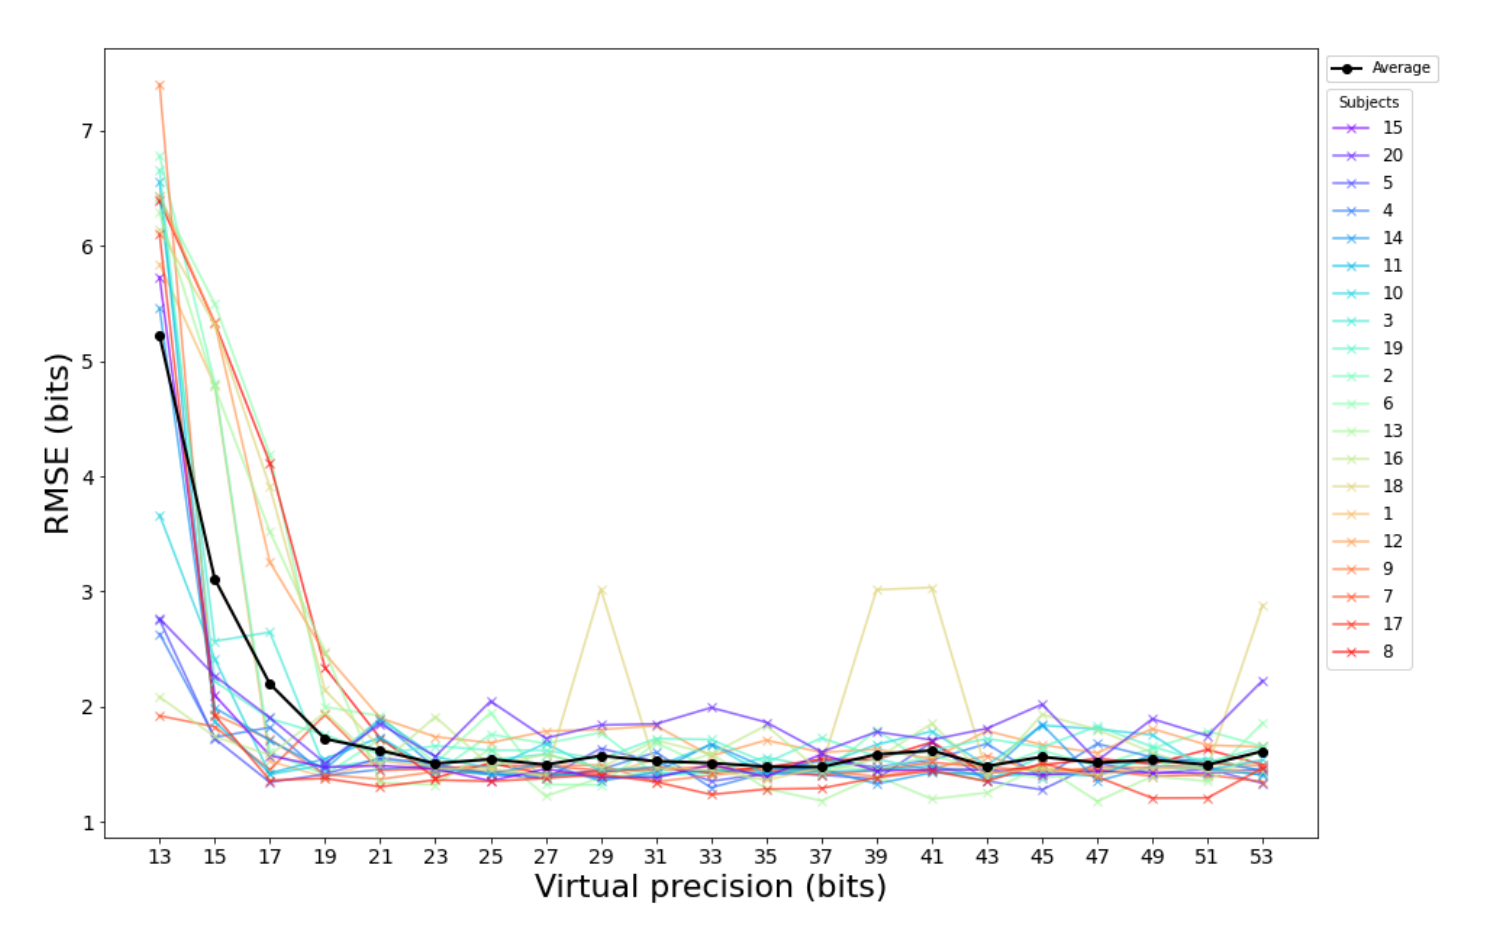
\includegraphics[width=\textwidth]{salari2021_vprec.png}
	\caption{RMSE values between OS and fuzzy libmath at each virtual precision (extracted from~\cite{Salari2021-kd}).}
	\label{fig:salari2021_vprec}
\end{figure}
	
Image smoothing is a commonly used method in neuroimaging pipelines.
It reduces the resolution of the data by combining close-by voxels.
Although in different ways, both image smoothing and reduced precision will affect
the precision of the data processed.
In a study by Molloy et al.~\cite{Molloy2014-oc}, the signal-to-noise ratio and
the fMRI signal's detection power could be improved by image smoothing. 
Moreover, they found that applying spatial smoothing did not significantly change the
results for functional connectivity when finding ROIs.
	
While image smoothing helps correct artifacts such as head motion, the smoothness might vary across the brain volume.
This can lead to confounds related to the smoothing of head motion.
Scheinost et al.~\cite{Scheinost2014-ds} propose a uniform spatial smoothing method
to reduce those confounds.
The authors found that uniformly smoothed volumes result in a significantly lower
correlation between regions and head motion.
Similar to other smoothing techniques, it could not remove all confounds; however, it remains promising. 
	
Overall, while some studies show concern about neuroimaging pipelines' numerical stability,
others suggest that a low amount of significant bits are used to perform calculations. 
Moreover, reduced precision techniques might have similar effects as spatial smoothingtechniques that are commonly used.
Additional research is needed to understand better the effects of applying reduced precision to neuroimaging pipelines.
